\documentclass[11pt,oneside,a4paper]{book}
\usepackage[a4paper]{geometry}
\usepackage[utf8]{inputenc}
\usepackage[T1]{fontenc}
\usepackage[english]{babel}
\usepackage{datetime}
\usepackage{textcomp}
%\usepackage{amsmath}
%\usepackage{amsfonts}
%\usepackage{amssymb}
%\usepackage[dvips]{graphicx}
\usepackage{lastpage}
%\usepackage{pst-node}
%\usepackage{bigdelim}
%\usepackage{multirow}
\usepackage{url}
\usepackage[printonlyused]{acronym}
\usepackage{algpseudocode}
\usepackage{algorithm}
\usepackage{tikz}
%\usepackage{tikz-timing}
\usepackage{bytefield}
\usepackage{srclist}
\usetikzlibrary{calc,trees,positioning,arrows,chains,shapes.geometric,%
    decorations.pathreplacing,decorations.pathmorphing,shapes,%
    matrix,shapes.symbols,fit}

\tikzset{
>=stealth',
  punktchain/.style={
    rectangle, 
    rounded corners, 
    % fill=black!10,
    draw=black, very thick,
    text width=10em, 
    minimum height=3em, 
    text centered, 
    on chain},
  line/.style={draw, thick, <-},
  element/.style={
    tape,
    top color=white,
    bottom color=blue!50!black!60!,
    minimum width=8em,
    draw=blue!40!black!90, very thick,
    text width=10em, 
    minimum height=3.5em, 
    text centered, 
    on chain},
  every join/.style={->, thick,shorten >=1pt},
  decoration={brace},
  tuborg/.style={decorate},
  tubnode/.style={midway, right=2pt},
}

\pgfdeclarelayer{background}
\pgfsetlayers{background,main}


\title{%
  Zeke\\
  A kernel for ARM processors
}
\author{% 
  Olli Vanhoja\\
  \texttt{olli.vanhoja@cs.helsinki.fi}
}
\date{%
\today
}

\pagestyle{plain}
\begin{document}
  \maketitle
  \tableofcontents
  
  \part{Introduction}

Zeke is a portable operating system for ARM processors.\footnote{Zeke is
portable to at least in a sense of portability between different ARM cores
and architectures.} Figure \ref{figure:zeke} illustrates architectural layers
of Zeke. Scope of Zeke project is to implement a portable
Unix-like\footnote{Project is aiming to implement the core set of kernel
features specified in \ac{POSIX} standard.} operating system from scratch that
is optimized for ARM architectures and is free of legacy.

In addition to portability another goal has been configurability and adjustable
footprint. This is achieved by modular kernel architecture and compile time
configuration.

\begin{figure}
  \pgfdeclarelayer{background}
\pgfsetlayers{background,main}

\definecolor{mybluei}{RGB}{124,156,205}
\definecolor{myblueii}{RGB}{73,121,193}
\definecolor{mygreen}{RGB}{202,217,126}
\definecolor{mypink}{RGB}{233,198,235}

% this length is used to control the width of the light blue frame
% for the upper part of the diagram
\newlength\myframesep
\setlength\myframesep{8pt}

\pgfkeys{
    /tikz/node distance/.append code={
        \pgfkeyssetvalue{/tikz/node distance value}{#1}
    }
}

\newcommand\widernode[5][blueb]{
\node[
        #1,
        inner sep=0pt,
        shift=($(#2.south)-(#2.north)$),
        yshift=-\pgfkeysvalueof{/tikz/node distance value},
        fit={(#2) (#3)},
        label=center:{\sffamily\bfseries\color{white}#4}] (#5) {};
}

\begin{tikzpicture}[node distance=3pt,outer sep=0pt,
blueb/.style={
  draw=white,
  fill=mybluei,
  rounded corners,
  text width=2.5cm,
  font={\sffamily\bfseries\color{white}},
  align=center,
  text height=12pt,
  text depth=9pt},
greenb/.style={blueb,fill=mygreen},
]
\node[blueb] (init) {init};
\node[blueb,right=of init] (usr) {User Program};
\widernode{init}{usr}{libc}{libc};
\widernode{libc}{libc}{Syscall Interface}{syscall};
\widernode{syscall}{syscall}{Kernel Core}{kernel};
\node[blueb, right=of kernel](vfs) {VFS};
\node[greenb,below=of kernel] (hal) {HAL};
\node[greenb,right=of hal] (drv) {Drivers};
\begin{pgfonlayer}{background}
\draw[blueb,draw=black,fill=mybluei!40] 
  ([xshift=-\myframesep,yshift=3\myframesep]current bounding box.north west) 
    rectangle 
  ([xshift=\myframesep,yshift=-\myframesep]current bounding box.south east);
\end{pgfonlayer}
\path  let \p1=( $ (syscall.east) - (syscall.west) $ )
 in node[blueb,inner xsep=0pt,draw=black,fill=myblueii,below=4pt of current bounding box.south,text width=\x1+2*\myframesep+2\pgflinewidth] (HW) {Hardware};
\node[font=\sffamily\itshape\color{white},above=of init] {Zeke};
\end{tikzpicture}
  \centering
  \caption{Zeke: a Portable Operating System.}
  \label{figure:zeke}
\end{figure}

\section*{List of Abbreviations and Meanings}

\begin{acronym}[UniversalSpacer]
\acro{POSIX}[POSIX]{Portable Operating System Interface for uniX\acroextra{ is a
  family of standards specifying a standard set of features for compatibility
  between operating systems.}}

\acro{vfs}[VFS]{Virtual File System\acroextra{.}}
\acro{inode}[inode]{\acroextra{inode is the file index node in Unix-style file
  systems that is used to represent a file file system object.}}
\acro{vnode}[vnode]{\acroextra{vnode is like inode but it's used as an
  abstraction level for compatibility between different file systems in Zeke.
  Particularly it's used at VFS level.}}
\acro{ramfs}[ramfs]{RAM file system\acroextra{.}}

\acro{dynmem}[dynmem]{(dynamic memory)\acroextra{ is the block memory allocator
  system in Zeke, allocating in 1 MB blocks.}}
\acro{vralloc}[VRAlloc]{Virtual Region Allocator\acroextra{.}}

\acro{PUnit}[PUnit]{a portable unit testing framework for C\acroextra{.}}
\acro{GCC}[GCC]{GNU Compiler Collection\acroextra{.}}
\acro{GLIBC}[GLIBC]{The GNU C Library\acroextra{.}}
\acro{CPU}[CPU]{Central Processing Unit\acroextra{ is, generally speaking, the
  main processor of some computer or embedded system.}}

\acro{MMU}[MMU]{Memory Management Unit\acroextra{.}}
\acro{DMA}[DMA]{Direct Memory Access\acroextra{ is a feature that allows
 hardware subsystems to commit memory transactions without \acsu{CPU}'s
 intervention.}}
\end{acronym}
  \part{Memory Management}

\chapter{Subsystem Overview}

This subsection briefly introduces the architectural layout of memory management
in Zeke at very generic level. Specifically we do not cover memory map layout or
anything hardware specific things here.

Zeke as well as most of major operating systems does its memory management and
mapping in multiple stages. In the kernel stages are built into following layers
of abstraction \ac{MMU} abstraction, \verb+dynmem+ handling dynamic allocation
of contiguous blocks of memory and \verb+kmalloc+ that allocates memory for the
kernel itself. These are the most important parts of the memory management in
Zeke as other parts of the kernel are only utilizing these to allocate or map
memory for use anywhere in the system.

Figure \ref{figure:mm_layers} shows the memory management stack from
top to bottom.

\begin{figure}
  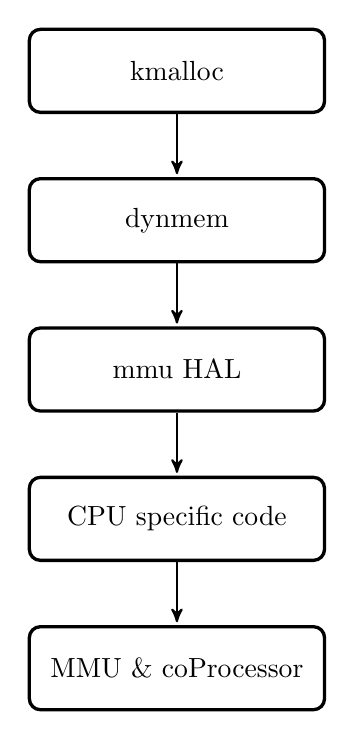
\begin{tikzpicture}
  [node distance=.8cm,
  start chain=going below,]
  	%\node[punktchain, join] (vfs)     {vfs};
	%\node[punktchain, join] (ramfs)   {ramfs};
    %\begin{scope}[start branch=ofsb]
   	%	\node[punktchain, on chain=going right] (ofs) {some other FS};
    %\end{scope}
    \node[punktchain, join] (kmalloc) {kmalloc};
    \node[punktchain, join] (dynmem)  {dynmem};
    \node[punktchain, join] (mmu)     {mmu HAL};
    \node[punktchain, join] (cpusp)   {CPU specific code};
    \node[punktchain, join] (hw)      {MMU \& coProcessor};
    %
    %\draw[|-,-|,->, thick,] (vfs.south) |-+(0,-1em)-| (ofs.north);
  % Now, let us add some braches. 
  %\draw[tuborg, decoration={brace}] let \p1=(ramfs.north), \p2=(kmalloc.south) in
  %  ($(2, \y1)$) -- ($(2, \y2)$) node[tubnode] {Scope of this document.};
  \end{tikzpicture}
  \centering
  \caption{Kernel layers from kmalloc to physical \acs{CPU} level.}
  \label{figure:mm_layers}
\end{figure}

\begin{description}
\item[kmalloc] is a malloc-like interface for allocating arbitrary sized blocks
  of memory.
\item[dynmem] is a block allocator that always allocates memory in block size of
  $1 \:\textrm{MB}$. See fig. \ref{figure:dynmem_blocks}.
\end{description}

Lets assume that some part of the kernel needs a new chunk of memory for some
temporal use, there is no more space left at any of the higher levels and most
importantly the code uses \verb+kmalloc+ to allocate the block. What happens
next is that memory allocation request is eventually passed to dynmem memory
allocator.

dynmem tries to locate the first free memory region in the dynmem memory section
that satisfies the condition
$\textrm{requested size} \le n \times 1 \:\textrm{MB}$. If dynmem finds a free
region it is then reserved and returned to \verb+kmalloc+. \verb+kmalloc+ will
then allocate memory from that and possibly other closely located reservations
for the original caller by using its own algorithm, which is at the moment quite
naive first fit algorithm.

kmalloc stores its linked list of reserved and free blocks in the same memory
that is used to allocate memory for its clients. Listing \ref{list:mblockt}
showsthe \verb+mblock_t+ structure definition used internally in kmalloc for
linking blocks of memory.

\begin{figure}
  \newcommand{\colorbitbox}[3]{%
\rlap{\bitbox{#2}{\color{#1}\rule{\width}{\height}}}%
\bitbox{#2}{#3}}

\definecolor{lightgreen}{rgb}{0.64,1,0.71}
\definecolor{lightred}{rgb}{1,0.7,0.71}

\begin{bytefield}[boxformatting={\centering\small},bitwidth=\widthof{Kernel~}]{4}
  \bitheader[endianness=little]{0-3} \\
  \colorbitbox{lightred}{1}{Kernel} &
  \colorbitbox{lightgreen}{1}{} &
  \colorbitbox{lightred}{2}{User} &
\end{bytefield}
  \centering
  \caption{Example of reserved dynmem regions.}
  \label{figure:dynmem_blocks}
\end{figure}

\lstinputlisting[label=list:mblockt,caption=kmalloc mblock\_t struct definition.]{mem/mblock_t.c}

\chapter{kmalloc}
The current implementation of the generic kernel memory allocator is largely
based on tutorial written by Marwan Burrelle\cite(Burelle:malloc).

\section{Brief Description}

The current kernel memory allocator implementation is somewhat naive and
exploits some very simple techniques like the first fit algorithm for allocating
memory.

Idea of the first fit algorithm is to find a first large enough free block of
memory from an already allocated region of memory. This is done by traversing
the list of memory blocks and looking for sufficiently large block. This is
ofcourse quite suboptimal and better solutions has to be considered.

When a large enough block is found it's splitted in two halves so that the left
one corresponds to requested size and the right block is left free. All data
blocks are aligned to 4 byte access.

Fragmentation of memory blocks is tried to keep minimal by merging newly freed
block with neighbouring blocks. This will at least keep all free blocks between
reserved blocks free but it doesn't help much if there is allocations of
different sizes that are freed independently. So current implementation is very
suboptimal also in this area.

When kmalloc is out of (large enough) memory blocks it will expand its memory
usage by allocating a new region of memory from dynmem. Allocation is done in
1 MB blocks (naturally) and always rounded  to a next 1 MB.

\begin{verbatim}
    +-+------+-+---------+-+-------+
    |d|      |d|         |d|       |
    |e| DATA |e|  FREE   |e| DATA  |
    |s|      |s|         |s|       |
    |c|      |c|         |c|       |
    +-+------+-----------+-+-------+
\end{verbatim}

Descriptors are used to store the size of the data block, reference counters and
pointers to neighbouring block descriptors.


\section{Suggestions for Further Development}

\subsection{Memory allocation algorithms}

Current implementation of kmalloc relies on first-fit algorithm and variable
sized blocks, that are processed as a linked list, which is obviously inefficient.

One possible improvement could be adding a second data structure that would
maintain information about free memory blocks that could be used to store the
most common object sizes. This data structure could be also used to implement
something like best-fit instead of first-fit and possibly with even smaller
time complexity than the current implementation.

\begin{eqnarray}
\mathrm{proposed\_size} &=& \mathrm{req\_size}
  + \frac{\mathrm{curr\_size}}{\mathrm{req\_size}} \mathrm{o\_fact}
  + \frac{\mathrm{curr\_size}}{o\_div}.
\end{eqnarray}

\begin{algorithm}
  \caption{krealloc over commit}
  \label{algo:realloc_oc}
  \begin{algorithmic}
      \If{$\mathrm{req\_size} > \mathrm{proposed\_size}$}
        \State $\mathrm{new\_size} \gets \mathrm{req\_size}$
      \Else
        \If{$\mathrm{limit}_{min} < 4 \frac{proposed\_size}{req\_size} < \mathrm{limit}_{max}$}
          \State $\mathrm{new\_size} \gets \mathrm{proposed\_size}$
        \Else
          \State $\mathrm{new\_size} \gets \mathrm{max(req\_size, curr\_size})$
        \EndIf
      \EndIf
  \end{algorithmic}
\end{algorithm}

This is however completely untested and intuitively derived method but it
seems to give a nice looking curves for hypothetical memory allocations as seen
in figure \ref{figure:realloc}.

\begin{figure}
  \center
  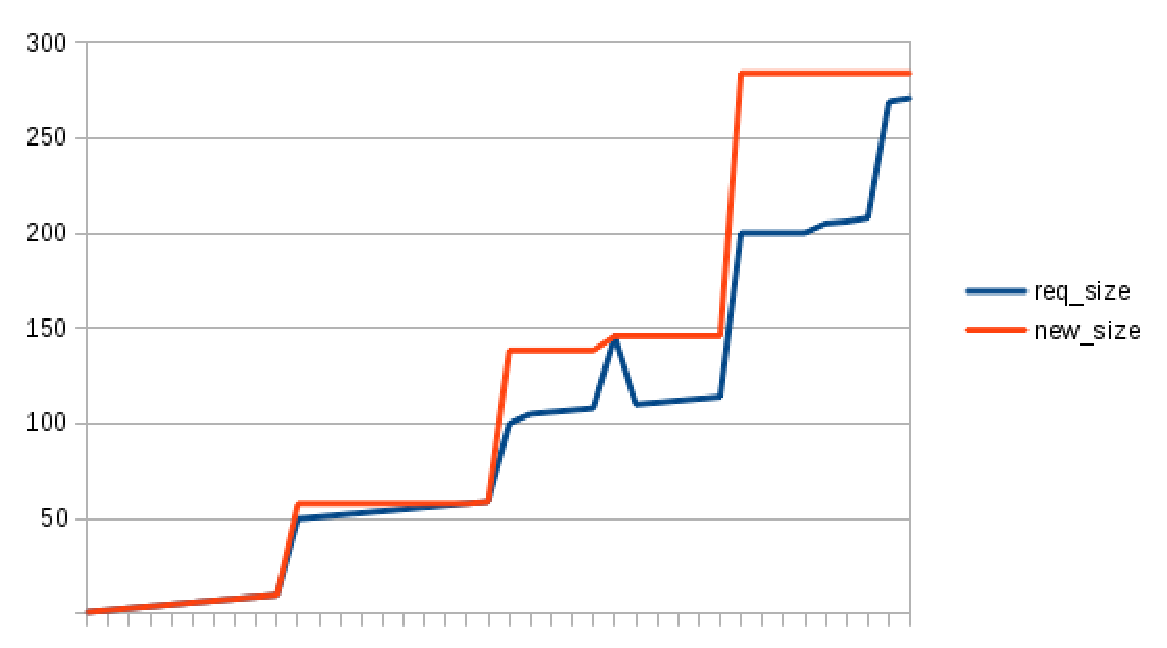
\includegraphics[width=10cm]{pics/realloc}
  \caption{New realloc method.}
  \label{figure:realloc}
\end{figure}

\chapter{Virtual Memory}
\chapter{Virtual Memory}

\section{Introduction to vmem in Zeke}

Every process has its own master page table and varying number of L2 page
tables. Kernel has its own master page table too. Static/fixed entries are
copied to all master page tables created. Process shares its master page
table with its childs.

Process page tables are stored in dynmem area.

ARM note: Only 4 kB pages are used with L2 page tables so XN (Execute-Never) bit
is always usable also for L2 pages.

\subsection{Domains}

See \verb+MMU_DOM_xxx+ definitions.

\subsection{Virtual memory abstraction levels}

\begin{figure}
\begin{verbatim}
U                      +---------------+
S                      |    malloc     |
R                      +---------------+
-------------------------------|-----------------
K   +---------------+  +---------------+
E   |    kmalloc    |  |    process    |
R   +---------------+  +---------------+
N           |     /\    |      |
E           |     |    \/      |
L           |  +--------+   +----+
            |  |vralloc |---| vm |
            |  +--------+   +----+
            |     |            |
           \/    \/           \/
    +---------------+     +----------+
    |    dynmem     |-----| ptmapper |
    +---------------+     +----------+
            |                  |
           \/                  |
    +---------------+          |
    |    mmu HAL    |<----------
    +---------------+
            |
    +-----------------------+
    | CPU specific MMU code |
    +-----------------------+
------------|------------------------------------
    +-------------------+
    | MMU & coProcessor |
    +-------------------+
\end{verbatim}
\caption{Virtual memory related subsystems in Zeke.}
\label{figure:vmsubsys}
\end{figure}

See figure \ref{figure:vmsubsys}.

\begin{itemize}
  \item \verb+kmalloc+  - is a kernel level memory allocation service, used
                        solely for memory allocations in kernel space.
  \item \verb+vralloc+  - VRAlloc is a special memory allocator targetted to
                        allocate blocks of memory that will be mapped in virtual
                        address space of processes, it returns \verb+vm_region+
                        structs instead of just base address of the allocation.
  \item \verb+dynmem+   - is a dynamic memory allocation system that allocates
                        \& frees contiguous blocks of physical memory.
  \item \verb+ptmapper+ - owns the statically created page tables (particularly
                        the master page table) and regions, and is also used to
                        allocate new page tables from the page table region.
  \item \verb+vm+       - vm runs various checks on virtual memory access,
                        copies data between user land and kernel space and
                        allocates memory for processes.
  \item mmu HAL -       is the abract MMU interface provided by \verb+mmu.h+
                        and \verb+mmu.c+.
  \item CPU specific MMU code is the module responsible of configuring the
        physical MMU layer and implementing the interface prodived by
        \verb+mmu.c+
\end{itemize}



  \part{File System}

\chapter{File System Abstraction}

\section{General Principles}

During this part of the document terms \acs{vnode} and \acs{inode} are
sometimes used interchangeably. Historically inode was a way to index files
in Unix-style file systems.\cite{Wikipedia:inode} While Zeke continues this
fashion it adds a concept of vnodes that are used as an abstraction level
between actual file systems and \acf{vfs}. This is done mostly in the same way
as on most of modern Unices today.

In Zeke vnodes are always used as a primary access method to the files in
a file system, inodes are only accessed internally within the file system
implementation code if the file system supports those. Expected behavior is
that a vnode and a vnode number exist in the system as long as some process owns
a reference to that vnode. After there is no more references to a vnode it's
not guaranteed that the vnode exist in the memory and it cannot be retrieved
by using its vnode number. In fact normally vnodes can't be accessed by their
vnode number but a vnode number is guaranteed to be unique within a one file
system, superblock + vnode, but same vnode might be in use with another fs and
it can be reused.

To simplifify understanding how vfs works in Zeke it can be described as an
object storage where file objects are first searched, found and the associated
(open) with a process. When a file is opened the process owns a pointer to the
file descriptor that contains some state information and pointer to the actual
file vnode. The vnode of the file is itself an object that knows where contents
of the file is stored (physical file system, superblock pointer) and who knows
how to manipulate the data (pointer to the vnode operations struct). In fact
vnode number itself is pretty much redundant and legacy information for Zeke
that is only provided for compatibility reasons, the actual access method is
always by a pointer reference to an object.

\section{Kernel Interface}

Kernel interface to the actual file system drivers and file system superblocks
is built around virtual function structs defined in \acs{vfs} header file
\verb+fs.h+ and some user space header files defining unified data types.

A new file system is first registered to the kernel by passing a pointer to
fs struct that is a complete interface for mounting a new superblock and
interacting with the file system (note the difference between a file system
(driver) and a file system superblock that is referencing to the actual data
storage, while fs driver is accessing the superblock. The file system struct
is shown in \ref{list:fs}.

When superblock is mounted a superblock struct pointer is returned. This pointer
servers as the main interface to the newly mounted file system. Superblock is
defined as in listing \ref{list:fs_sb}. By using superblock function calls it's
possible to get direct references to vnodes and \acs{vnode} operations e.g. for
modifying file contents or adding new hard links to a directory node.

\lstinputlisting[label=list:fs,caption=fs struct definition.]{fs/fs.c}
\lstinputlisting[label=list:fs_sb,caption=superblock struct definition.]{fs/fs_superblock.c}

\section{VFS hash}

\verb+vfs_hash+ is an optional hashmap used for vnode caching for physically
slow file systems. VFS itself doesn't use this caching for any purpose so
it is completely optional to insert anything into there.

\chapter{ramfs}
\section{Overall description}

The purpose of the \acs{ramfs} is to provide a storage in RAM for temporary
files. This is important in user scope where there might be no other writable
storage medium available on some embedded platform. In addition to storage
for temporary files in user scope ramfs could be useful to store kernel files
as well, e.g. init can be unpacked from kernel to ramfs and then executed.

In the future ramfs code might be also useful for \acs{vfs} caching, so that
changes to a slow medium could be stored in ramfs-like structure and synced
later.

Ramfs should implement the same \acs{vfs} interface as any other regular
file system for Zeke. This ensures that the same POSIX compliant file
descriptor interface\footnote{POSIX file API is not actually yet implemented.}
can be used for files stored to ramfs as well as to any other file system.

\section{Structure of ramfs}

Data in Ramfs is organized by inodes, \acs{inode} can contain either a file or
directory entries, which means that an inode can be either files or directories.
Maximum size of a mounted ramfs is limited by size of \verb+size_t+ type.
Maximum size of a file is limited by size of \verb+off_t+ type. Figure
\ref{figure:inodes} shows a high level representation of how inodes are
organized and linked in ramfs to form directory tree with files and directories.

Contents of a file is stored in blocks of memory that are dynamically allocated
on demand. Block size is selected per file so all blocks are equal size and
block pointer array (\verb+in.data+) is expanded when new blocks are allocated
for a file. Figure \ref{figure:file} shows how memory is allocated for a file
inode.

Directory in ramfs is stored similarly to a file but \verb+in.dir+ (union with
\verb+in.data+) is now constant in size and it's used as a hash table which
points to chains of directory entries (directory entry arrays). If two files are
mapped to a same chain by hash function then the corresponding chain array is
re-sized so that the new entry can be added at the end of array. This means that
lookup from a directory entry chain is quite cache friendly and can usually
avoid fragmentation in memory allocation. Figure \ref{figure:dir} represents a
directory inode containing some directory entries.

\begin{figure}
  \center
  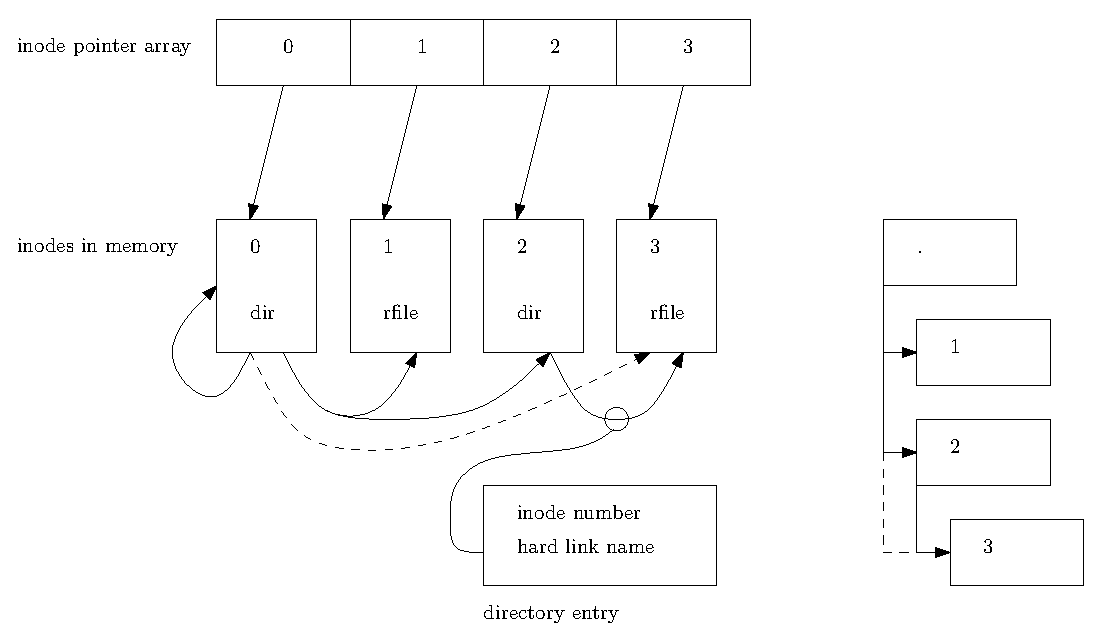
\includegraphics[width=15cm]{pics/inodes}
  \caption{Mounted ramfs with some inodes.}
  \label{figure:inodes}
\end{figure}

\begin{figure}
  \center
  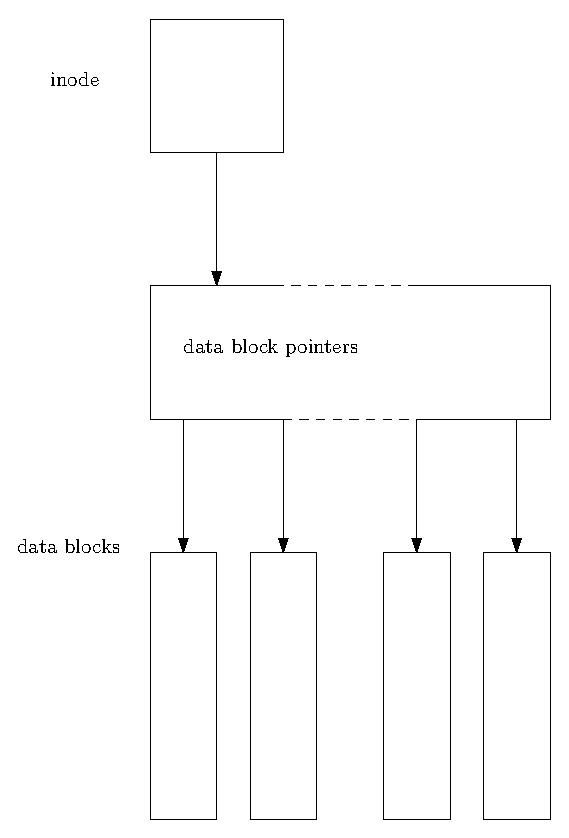
\includegraphics[width=7cm]{pics/file}
  \caption{Structure of a file stored in ramfs.}
  \label{figure:file}
\end{figure}

\begin{figure}
  \center
  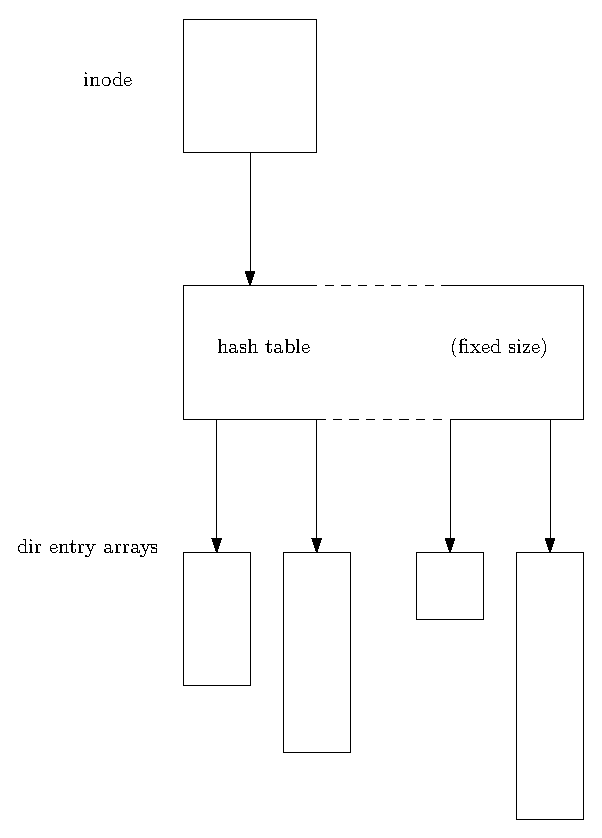
\includegraphics[width=7cm]{pics/dir}
  \caption{Directory containing some directory entries in ramfs.}
  \label{figure:dir}
\end{figure}


\section{Time Complexity and Performance Analysis}

\subsection{Mount}

When a new ramfs superblock is mounted it's appended to the end of the global
superblock list. Time complexity of this operation is $O(n)$ as there is no
information about the last node in the list. However this is not a major
problem because new mounts happen relatively rarely and other operations during
the mounting process will take much more time than traversing a super block list
of any practical length. Those other operations includes allocating memory for
inode array, allocating memory for inode pool and initializing some data
structures etc.

\subsection{Get vnode by vnode number}

Index nodes are stored in contiguous array as shown in figure
\ref{figure:inodes}. This trivially means that a vnode can be always fetched
from mounted ramfs in $O(1)$ time as it's only a matter of array indexing.

\subsection{Lookup vnode by filename}

File lookup on ramfs level is implemented only on single directory vnode level
and sub-directory lookup must be then implemented on \acs{vfs} level i.e. lookup
function for a vnode can only lookup for entries in the current directory
vnode. A file lookup is made by calling \verb+vnode->vnode_ops->lookup()+.    

Directory entries are stored in chained hash tables as shown in figure
\ref{figure:dir}. It can be easily seen that usually a chain array contains only
a single entry and therefore lookup is $O(1)$. In sense a of performance and
efficiency of a chain array with length greater than zero is more complex.
Trivially lookup from array is of course $O(n)$. What is interesting here is
how CPU caching works here. Even though directory entries are different in size
they are all stored in contiguous memory area and can be loaded to CPU cache
very efficiently, whereas many other data structures may lead to several
non-contiguous memory allocations that will pollute the caching and slow down
the lookup if there is only few entries. That said the current implementation of
directory entry storage seems almost perfect solution if amount of directory
entries is moderate and hash functions is good enough.\cite{Wikipedia:htable}

\subsection{Data by vnode}

Data stored in file inodes is accessed by calling
\verb+vnode->vnode_ops->read()+ and \verb+vnode->vnode_ops->write()+. Arguments
for both contains a pointer to the vnode, offset where to start reading or
writing from, byte count and a pointer to a buffer. Data structuring of a file
vnode was illustrated in figure \ref{figure:file}.

Pointer to a block of data by \verb+offset+ is calculated as shown in equation
\ref{eqn:dpointer}, where data is the data block pointer array. Length of
data pointer by the pointer is calculated as shown in equation \ref{eqn:dlen}.

\begin{eqnarray}
  \textrm{block} &=& \textrm{data} \left[ \frac{\textrm{offset} -
    (\textrm{offset} \& (\textrm{blksize} - 1))}{\textrm{blksize}}
    \right] \\
  \textrm{p}     &=& \textrm{block} \left[ \textrm{offset} \& (\textrm{blksize} - 1)
    \right] \label{eqn:dpointer} \\
  \textrm{len}  &=& \textrm{blocksize} - (\textrm{offset} \& (\textrm{blksize} - 1)) \label{eqn:dlen}
\end{eqnarray}

\subsection{Create a vnode}

Normally when a new inode is created it can be taken from the inode pool and
inserted at empty location on inode array. Average case can be considered to be
$O(1)$ then.

Lets consider a case where a new vnode is created and inserted to the index node
array but it's already full. A call to \verb+krealloc()+ will be issued and the
worst case of reallocation of a memory location may require to create a copy
of the whole index node array to a new location. This means that the worst case
time complexity of a vnode creation is relative to size of the array, so its
$O(n)$.

\subsection{Summary}

\begin{table}
  \caption{Summary of time complexity of ramfs functions.}
  \label{table:complexity}
  \begin{tabular}{lcc}
    Function & Average time complexity & Worst case time complexity \\
    \hline
    mount                 & $O(n)$ & $O(n)$ \\
    vnode by vnode number & $O(1)$ & $O(1)$ \\
    vnode by filename     & $O(1)$ & $O(n)$ \\
    data by vnode         & $O(1)$ & $O(1)$ \\
    create a new vnode    & $O(1)$ & $O(n)$
  \end{tabular}
\end{table}


\section{Performance Testing}

Automated performance tests were implemented the same way as unit tests.
Ramfs performance tests are in \verb+test_ramfsperf.c+ file.

\subsection{Test Results}

\subsection{Hard link operations}

Performance of hard link operations is tested in \verb+test_dehtableperf.c+.

Figure \ref{figure:dhlink_perf} shows performance measurements from
\verb+test_link_perf()+ test. In this test number of randomly named nodes are
added at every point and total time of adding those links is measured.
Name collisions are not handled but just appended to the chain array.
It seems that total time of \verb+dh_link()+ calls is almost flat but
it then starts to smoothly transform to something that is almost linearly
relative to the amount of links added. Calls to \verb+kmalloc()+ and
\verb+krealloc()+ seems to add some random behavior to link times.

Lookup tests were performed with \verb+test_lookup_perf()+ test and illustrated
in figure \ref{figure:dhlookup_perf}. The test works by first adding certain
amount of randomly named links and then trying to lookup with another set of
randomly selected names. Hit percentage is named as "\% found" in the plot and
lookup time is the mean of 100 random lookups. Lookup function seems to behave
quite linearly even though there is some quite strange deviation at some link
counts.

Even though lookups seems to be in almost linear relationship with the link
count of the directory entry hash table it doesn't mean lookups are slow.
Even with 20000 links average lookup takes only $45\:\mu s$ and it's very
rare to have that many directory entries in one directory.

\begin{figure}
  \includegraphics[width=15cm]{plots/dh_link}
  \centering
  \caption{Directory entry hash table link performance.}
  \label{figure:dhlink_perf}
\end{figure}

\begin{figure}
  \includegraphics[width=15cm]{plots/dh_lookup}
  \centering
  \caption{Directory entry hash table lookup performance.}
  \label{figure:dhlookup_perf}
\end{figure}

\subsubsection{File operations}

Performance tests for file operations were performed on the universal target
where kmalloc uses malloc instead of dynem block allocator, this in fact may
make some of the result unreliable.

\begin{tabular}{l r@{.}l}
\textbf{Operation} &
\multicolumn{2}{c}{\textbf{Transfer speed (MB/s)}} \\
\hline
\textbf{Single write (100 MB)} && \\
new file      & 21&62 \\
existing file & 1694&92 \\
read          & 1098&90 \\
\textbf{Sequential writes} && \\
new file      & 9&06 \\
existing file & 335&80 \\
read          & 426&22 \\
\end{tabular}

\subsubsection{ramfs write/read performance}

Write and read performance testing is somewhat biased by the underlying kernel
even though we have our own memory allocator in place. Actually kmalloc may
make things work even worse because it's optimized for different kind of
suballocator that is not present on API level of Linux. So I think this is a
major cause for very poor memory allocation and first pass write performance
to the allocated blocks of memory, although kmalloc it self is quite inefficient
too.


\section{Suggestions for Further Development}

\subsubsection{Directories}

Directory entry lookup tables (hash tables) could be made variable in size.
This would make use of directory entry chains less frequent and greatly improve
performance of large directories while still maintaining small footprint for
small directories containing only few entries. At minimum this would only
require a function pointer to the current hash function in the inode. There is
no need to store the size of current hash table array in variable because it can
be determined by comparing the function pointer. So overhead of this improvement
would be size of \verb+size_t+ per directory and one more dereference per lookup.


\chapter{devfs}
\section{Introduction}

Devfs inherits ramfs and creates an abstraction layer between device drivers
and device driver abstraction layers. Essentially devfs creates a file
abstraction with vfs read() and write() functions that communicates with the
actual device driver.

\section{Device creation process}

Device registration with devfs starts from static init function of a subsystem,
device detection routine or some other triggering method. The device
identification/creation function shall, by some way, create a \verb+dev_info+
struct that describes the device and provides necessary function pointers for
reading and writing. Then \verb+make_dev(devXXX_info, 0, 0, 0666)+ is called
to register the device created. \verb+make_dev()+ then creates a fs node that is
contains a pointer to the provided \verb+dev_info+ in \verb+vn_specinfo+ of the
device.

There is some notable differences between devfs implementation of Zeke and other
common devfs or device abstractions in some other operating systems,
particularly Unices. First of all we don't use majorminor combination as a
device idetentifier, it's only provided for compatibility reasons and not used
for anything actually.\footnote{Some drivers may still use those internally but
there is no external interface provided. Uart is one of those using minor
numbers for internal indexing.} So devices can't be accessed by creating
a device file anywhere in the system, device files in Zeke are very special and
only ones that are created with \verb+make_dev()+ are valid, since the object
oriented model of Zeke VFS.

Another difference is that Zeke does not have character and block device
access modes/file types like most of traditional Unices. Zeke can support
buffered writes but it's always hidden from the user space. In practice,
it means that every user reading from a device file will always see the
same state, eg. if one process would write by using block device and another
one reading character device, the latter one would get either old data or
corrputed data. In fact there is no reason to have different file types for
different device types, block device files were designed to be a special file
type for hard disks, for some reason, but it doesn't make any sense to do it
that way in a modern kernel.\cite{Kamp:rethinkdev} Thus block device files are
not supported in Zeke and buffered access is not implemented but technically
supported inside the kernel.

\section{UART devices}

UART devices are handled by UART submodule (\verb+kern/hal/uart.c+) so that
common code between UART implementations can be shared and tty numbering can
be centrally organized. To register a new UART port the device driver has to
allocate a new \verb+uart_port+ structure and pass it to
\verb+uart_register_port()+ which finally registers the a new device file for
the port.

\begin{figure}
  \center
  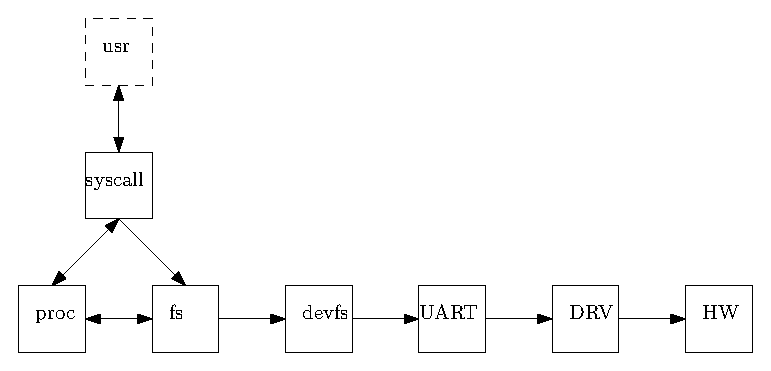
\includegraphics[width=9cm]{pics/uart}
  \caption{Communication between subsystems when a user process is writing to a UART.}
  \label{figure:dir}
\end{figure}



  
  \bibliography{ramfs.bib}{}
  \bibliographystyle{plain}

\end{document}